\section{解线性方程组的迭代法}
\subsection{迭代法的构造}
\begin{note}
    迭代法的基本思想:

    \[
        \boldsymbol{Ax}=\boldsymbol{b}\Leftrightarrow \boldsymbol{x}=\boldsymbol{Bx}+\boldsymbol{f}
    \]
    选取初始向量$x^{(0)}$,构造迭代格式:
    \[
        \begin{aligned}
            \boldsymbol{x}^{(1)} = \boldsymbol{Bx}^{(0)}+\boldsymbol{f}\\
            \boldsymbol{x}^{(2)} = \boldsymbol{Bx}^{(1)}+\boldsymbol{f}\\
            \vdots\\
            \boldsymbol{x}^{(k)} = \boldsymbol{Bx}^{(k-1)}+\boldsymbol{f}\\
        \end{aligned}
    \]
    两边取极限得到
    \[
        \boldsymbol{x}^* = \boldsymbol{Bx}^*+\boldsymbol{f}
    \]
\end{note}
\begin{note}
    迭代法构造的一般原则:

    将系数矩阵分解为
    \[
        \boldsymbol{A} = \boldsymbol{M}-\boldsymbol{N}
    \]
    故而有
    \[
        \boldsymbol{Ax}=\boldsymbol{b}\Leftrightarrow \boldsymbol{Mx}=\boldsymbol{Nx}+\boldsymbol{b}
    \]
    从而方程组等价化为
    \[
        \boldsymbol{x} =\boldsymbol{M}^{-1}\boldsymbol{Nx}+\boldsymbol{M}^{-1}\boldsymbol{b}
    \]
    需要满足以下条件
    \begin{itemize}
        \item $\boldsymbol{M}$非奇异
        \item $\boldsymbol{M}^{-1}$容易求
    \end{itemize}
\end{note}
迭代法的收敛性

\begin{theorem}[迭代法基本定理]
    对于任意的初始向量$\boldsymbol{x}^{(0)}$,迭代法构
    \[
        \boldsymbol{x}^{(k)} = \boldsymbol{Bx}^{(k-1)}+\boldsymbol{f}
    \]
    收敛的充分必要条件为
    \[
        |\lambda_{i}(\boldsymbol{B})|<1,\quad (i = 1,\cdots,n)
    \]
    或者
    \[
        \rho(\boldsymbol{B})<1
    \]
\end{theorem}
\begin{example}
    用迭代法求解下列方程组
    \[
        \begin{cases}
            8x_1-3x_2+2x_3=20\\
            4x_1+11x_2-x_3=33\\
            6x_1+3x_2+12x_3=36
        \end{cases}
        \quad
        \begin{pmatrix}x_1\\x_2\\x_3\end{pmatrix}
        =
        \begin{pmatrix}3.0000\\2.0000\\1.0000\end{pmatrix}
    \]
    \begin{solution}
        将系数矩阵分解为
        \[
            \begin{pmatrix}
                8 & -3 & 2\\
                4 & 11 & -1\\
                6 & 3 & 12
            \end{pmatrix} = 
            \begin{pmatrix}
                8 &  & \\
                 & 11 & \\
                 &  & 12
            \end{pmatrix}-
            \begin{pmatrix}
                0 & 3 & -2\\
                -4 & 0 & 1\\
                -6 & -3 & 0
            \end{pmatrix}
        \]
        从而构造迭代法
        \[
            \boldsymbol{x}^{k} = 
                \boldsymbol{M}^{-1}\boldsymbol{N}\boldsymbol{x}^{(k-1)}+\boldsymbol{M}^{-1}\boldsymbol{b}
        \]
    \end{solution}
\end{example}
\begin{theorem}
    对于任意的初始向量$\boldsymbol{x}^{(0)}$,若存在$\boldsymbol{B}$的某种范数$\parallel\cdot\parallel$,使得$\parallel \boldsymbol{B}\parallel=q<1$,则迭代法收敛,且
    \begin{enumerate}
        \item $\parallel \boldsymbol{x}^{(k)}-\boldsymbol{x}^{*}\parallel\leq\frac{q}{1-q}\parallel \boldsymbol{x}^{(k)}-\boldsymbol{x}^{(k-1)}\parallel;$
        \item $\parallel \boldsymbol{x}^{(k)}-\boldsymbol{x}^{*}\parallel\leq\frac{q^{k}}{1-q}\parallel \boldsymbol{x}^{(1)}-\boldsymbol{x}^{(0)}\parallel.$
    \end{enumerate}
\end{theorem}
\begin{proof}
    先证明1
    \[
        \begin{aligned}
            \parallel \boldsymbol{x}^{(k)}-\boldsymbol{x}^{*}\parallel&= \|\boldsymbol{B}(\boldsymbol{x}^{(k-1)}-\boldsymbol{x}^{*})\|\\
            &\leq \|\boldsymbol{B}\|\|(\boldsymbol{x}^{(k-1)}-\boldsymbol{x}^{*})\|\\
            & = \|\boldsymbol{B}\|\|(\boldsymbol{x}^{(k-1)}-\boldsymbol{x}^{k}) + (\boldsymbol{x}^{(k)}-\boldsymbol{x}^{*})\|\\
            & \leq \|\boldsymbol{B}\|\|(\boldsymbol{x}^{(k)}-\boldsymbol{x}^{(k-1)}) \| + \|\boldsymbol{B}\|\| (\boldsymbol{x}^{(k)}-\boldsymbol{x}^{*})\|\\
            & = q\|\boldsymbol{x}^{(k)}-\boldsymbol{x}^{(k-1)} \| + q\| \boldsymbol{x}^{(k)}-\boldsymbol{x}^{*}\|\\
        \end{aligned}  
    \]
    故而
    \[
        \parallel \boldsymbol{x}^{(k)}-\boldsymbol{x}^{*}\parallel\leq\frac{q}{1-q}\parallel \boldsymbol{x}^{(k)}-\boldsymbol{x}^{(k-1)}\parallel 
    \]

    再证明2
    \[
        \begin{aligned}
            \parallel \boldsymbol{x}^{(k)}-\boldsymbol{x}^{*}\parallel&\leq\frac{q}{1-q}\parallel \boldsymbol{x}^{(k)}-\boldsymbol{x}^{(k-1)}\parallel\\
            &\leq \frac{q^k}{1-q}\parallel \boldsymbol{x}^{(1)}-\boldsymbol{x}^{(0)}\parallel
        \end{aligned}
    \]
\end{proof}
\begin{example}
    对线性方程组
    \[
        \begin{pmatrix}3&2\\1&2\end{pmatrix}\begin{pmatrix}x_1\\x_2\end{pmatrix}=\begin{pmatrix}3\\-1\end{pmatrix}
    \]
    若用迭代法
    \[
        \boldsymbol{x}^{(k+1)}=\boldsymbol{x}^{(k)}+\alpha(\boldsymbol{A}\boldsymbol{x}^{(k)}-\boldsymbol{b})
    \]
    求解,则$\alpha\in$\sol{(-0.5,0)}时迭代收敛,$\alpha=$\sol{-0.4} 时迭代收敛最快。
    \begin{solution}
        由$\boldsymbol{x}^{(k+1)}=\boldsymbol{x}^{(k)}+\alpha(\boldsymbol{A}\boldsymbol{x}^{(k)}-b)$知道
        \[
            \boldsymbol{x}^{(k+1)}=(\alpha \boldsymbol{A}+\boldsymbol{I})\boldsymbol{x}^{(k)}-\alpha b
        \]
        求$\alpha \boldsymbol{A}+I$的谱半径$\rho$
        \[
            \begin{aligned}
                &\begin{vmatrix}
                    \lambda-3\alpha-1 & -2\alpha\\
                    -\alpha & \lambda-2\alpha-1
                \end{vmatrix}\\
                &=\lambda^2-(5\alpha+2)\lambda+(3\alpha+1)(2\alpha+1)-2\alpha^2\\
                &=\lambda^2-(5\alpha+2)\lambda+4\alpha^2+5\alpha+1\\
                &=[\lambda-(4\alpha+1)][\lambda-(\alpha+1)]
            \end{aligned}
        \]
        谱半径的图像$\rho = \max\left\{ |4\alpha+1|,|\alpha+1| \right\}$
        \begin{figure}[ht]
            \centering
            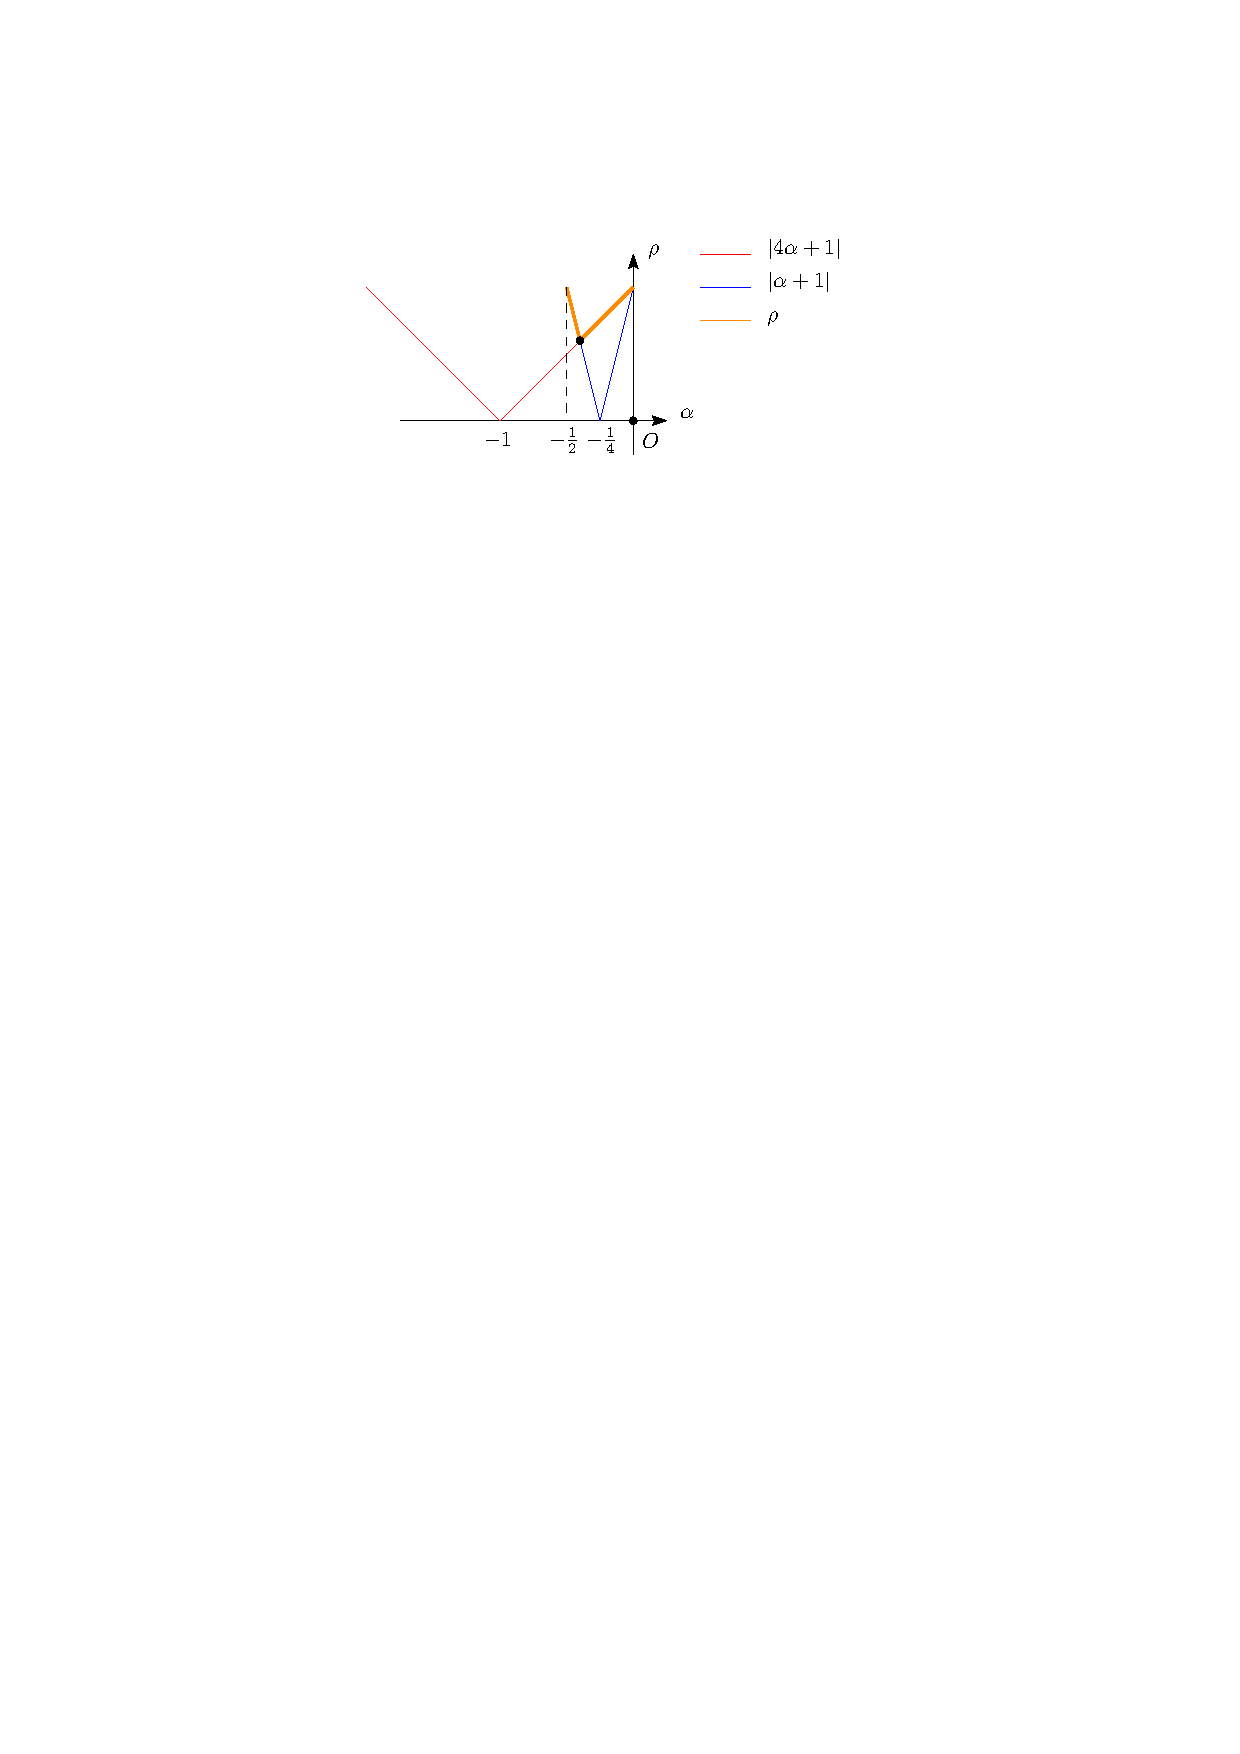
\includegraphics{image/迭代法rho-example.pdf}
        \end{figure}

        当$\alpha\in(-0.5,0)$时迭代收敛,$\alpha=-0.4$ 时迭代收敛最快
    \end{solution}
\end{example}
\subsubsection{Jacobi迭代法}
设$a_{ii}\neq 0,\,(i = 1,2,\cdots n),\,\boldsymbol{M} = \boldsymbol{D},\,\boldsymbol{N} = \boldsymbol{D}-\boldsymbol{A}$,有
\[
    \begin{array}{l}
        \boldsymbol{B}_{J} = \boldsymbol{D}^{-1}(\boldsymbol{D}-\boldsymbol{A}) = \boldsymbol{I}-\boldsymbol{D}^{-1}\boldsymbol{A} = \boldsymbol{D}^{-1}(\boldsymbol{L}+\boldsymbol{U})\\
        \boldsymbol{f} = \boldsymbol{D}^{-1}\boldsymbol{b}
    \end{array}
\]
\[
    \boldsymbol{x}^{(k+1)} = \boldsymbol{B}_{J}\boldsymbol{x}^{(k)}+\boldsymbol{f}
\]
\begin{theorem}[Jacobi迭代的收敛性定理]
    Jacobi迭代法收敛有以下结论
    \begin{itemize}
        \item Jacobi迭代法收敛的充分必要条件是
        \[
            \rho(\boldsymbol{B}_{J})<1        
        \]
        \item Jacobi迭代法收敛的充分条件是存在一种范数$\|\cdot\|$,使得$\|\boldsymbol{B}_{J}\|\leqslant 1$
    \end{itemize}
\end{theorem}
\subsubsection{Gauss-Seidel迭代法}
\[
    \begin{gathered}
        x_{1}^{(k+1)}=\frac{1}{a_{11}}(b_{1}-\sum_{j=2}^{n}a_{1j}x_{j}^{(k)}) \\
        \begin{aligned}x_{2}^{(k+1)}&=\frac{1}{a_{22}}(b_{2}-a_{21}x_{1}^{(k+1)}-\sum_{j=3}^{n}a_{2j}x_{j}^{(k)})\\&\cdots\cdots\end{aligned} \\
        x_{i}^{(k+1)}=\frac{1}{a_{ii}}(b_{i}-\sum_{j=1}^{i-1}a_{ij}x_{j}^{(k+1)}-\sum_{j=i+1}^{n}a_{ij}x_{j}^{(k)}) 
    \end{gathered}
\]
\[
    \boldsymbol{x}^{(k+1)} = \boldsymbol{G}\boldsymbol{x}^{(k)}+\boldsymbol{f}_{G}
\]
其中
\[
    \boldsymbol{G} = (\boldsymbol{D}-\boldsymbol{L})^{-1}\boldsymbol{U},\,\boldsymbol{f}_{G} = (\boldsymbol{D}-\boldsymbol{L})^{-1}\boldsymbol{b}
\]
\begin{theorem}[GS迭代的收敛性定理]
    GS迭代法收敛的充分必要条件是
    \begin{itemize}
        \item GS迭代法收敛的充分必要条件是
        \[
            \rho(\boldsymbol{G})<1        
        \]
        \item GS迭代法收敛的充分条件是存在一种范数$\|\cdot\|$,使得$\|\boldsymbol{G}\|\leqslant 1$
    \end{itemize}
\end{theorem}
\subsubsection{SOR}
\[
    \widetilde{x_i}^{(k+1)}=\frac1{a_{ii}}(b_i-\sum_{j=1}^{i-1}a_{ij}x_j^{(k+1)}-\sum_{j=i+1}^na_{ij}x_j^{(k)})
\]
\[
    \begin{aligned}
        x_{i}^{(k+1)}&=(1-\omega)x_{i}^{(k)}+\omega\widetilde{x}_{i}^{(k+1)}\\
        &=x_{i}^{(k)}+\omega\left(\widetilde{x}_{i}^{(k+1)}-x_{i}^{(k)}\right)\\
        &=(1-\omega)x_{i}^{(k)}+\frac{\omega}{a_{ii}}(b_{i}-\sum_{j=1}^{i-1}a_{ij}x_{j}^{^{(k+1)}}-\sum_{j=i+1}^{n}a_{ij}x_{j}^{^{(k)}})
    \end{aligned}
\]
其中$\omega$为可选择的松弛因子
\[
    \begin{array}{l}
        \boldsymbol{x}^{(k+1)} = (1-\omega)\boldsymbol{x}^{(k)}+\omega \boldsymbol{D}^{-1}\left( \boldsymbol{b}+\boldsymbol{L}\boldsymbol{x}^{(k+1)}+\boldsymbol{U}\boldsymbol{x}^{(k)} \right)\\
        (\boldsymbol{D}-\omega \boldsymbol{L})\boldsymbol{x}^{(k+1)} = [(1-\omega)\boldsymbol{D}+\omega \boldsymbol{U}]\boldsymbol{x}^{(k)} + \omega \boldsymbol{b}
    \end{array}
\]
表示为矩阵
\[
    \boldsymbol{x}^{(k+1)}=\boldsymbol{G}_\omega \boldsymbol{x}^{(k)}+\boldsymbol{f}_\omega 
\]
\[
    \boldsymbol{G}_\omega=(\boldsymbol{D}-\omega \boldsymbol{L})^{-1}[(1-\omega)\boldsymbol{D}+\omega \boldsymbol{U}]
\]
\[
    \boldsymbol{f}=\omega(\boldsymbol{D}-\omega \boldsymbol{L})^{-1}\boldsymbol{b}
\]
\begin{theorem}[(SOR方法收敛的必要条件)]
设解$\boldsymbol{Ax}=\boldsymbol{b}(\boldsymbol{A}\in\mathbb{R}^{n\times n})$的SOR方法收敛。则$0<\omega<2.$
\end{theorem}
\begin{proof}
    SOR法收敛就是$\rho(\boldsymbol{G}_\omega) <1$
    因为$\boldsymbol{G}_\omega = (D-\omega\boldsymbol{L})^{-1}[(1-\omega)\boldsymbol{D}+\omega\boldsymbol{U}]$
    \[
        |\det(\boldsymbol{D}-\omega \boldsymbol{L})| = \prod_{i = 1}^{n}|a_{ii}|
    \]
    \[
        |\det((1-\omega)\boldsymbol{D}+\omega \boldsymbol{U})| = |(1-\omega)^n|\prod_{i = 1}^{n}|a_{ii}|
    \]
    \[
        |\det (\boldsymbol{G}_{\omega})| = |(1-\omega)^n|\leq \rho(\boldsymbol{G}_{\omega})^{n}
    \]
    \[
        \begin{array}{l}
            |(1-\omega)|< \rho(\boldsymbol{G}_{\omega})<1\\
            -1<1-\omega<1\\
            0<\omega<2
        \end{array}
    \]
    证毕!
\end{proof}
\begin{note}
    关于解特殊方程组迭代法的收敛性
    \begin{definition}[对角占优]
        设$\boldsymbol{A}=(a_ij)\in\mathbb{R}^{n\times n}$,则
        \begin{itemize}
            \item 若$\mid a_{ii}\mid>\sum_{j=1}^{n}\mid a_{ij}\mid(i=1,2,\cdots,n)$,称$\boldsymbol{A}$为严格对角占优矩阵(或强占优阵)。
            \item 若$\mid a_ii\mid \geq \sum _{i= 1}^{n}\mid a_{ij}\mid ( j= 1, 2, \cdots , n)$, 且至少有一个不等式严格成立,则称$\boldsymbol{A}$为弱对角占优阵。
        \end{itemize}
    \end{definition}
    \begin{definition}[(可约与不可约阵)]
        设$\boldsymbol{A}=(a_{ij})\in\mathbb{R}^{n\times n}(n\geq2)$,如果存在置换矩阵 $\boldsymbol{P}$使
        \[
            \boldsymbol{P}^{\mathrm{T}}\boldsymbol{A}\boldsymbol{P}=\begin{pmatrix}\boldsymbol{A}_{11}&\boldsymbol{A}_{12}\\0&\boldsymbol{A}_{22}\end{pmatrix}
        \]
        其中$\boldsymbol{A}_{11}$为$r$阶方阵,$\boldsymbol{A}_{22}$为$n-r$阶方阵$(1\leq r<n)$,则称$\boldsymbol{A}$为可约矩阵;否则如果不存在这样的置换矩阵$\boldsymbol{P}$使上式成立,称$\boldsymbol{A}$为不可约阵.
    \end{definition}
    \[
        \boldsymbol{Ax} = \boldsymbol{b}\Rightarrow \boldsymbol{P}^{\mathrm{T}}\boldsymbol{A}\boldsymbol{P}\boldsymbol{P}^{\mathrm{T}}x = \boldsymbol{P}^{\mathrm{T}}\boldsymbol{b}
    \]
    \[
        \begin{pmatrix}\boldsymbol{A}_{11}&\boldsymbol{A}_{12}\\0&\boldsymbol{A}_{22}\end{pmatrix}\begin{pmatrix}
            y_1\\y_2
        \end{pmatrix} = \begin{pmatrix}
            \boldsymbol{C}_1\\\boldsymbol{C}_2
        \end{pmatrix}
    \]
\end{note}
\begin{theorem}
    设$\boldsymbol{Ax}=\boldsymbol{b}$,$\boldsymbol{A}=(a_{ij})\in\mathbb{R}^{n\times n}$,
    \begin{itemize}
        \item 如果$\boldsymbol{A}$为严格对角占优阵,则解方程组$\boldsymbol{Ax}=\boldsymbol{b}$的J法及GS法均收敛.
        \item 如果$\boldsymbol{A}$为弱对角占优阵且不可约阵,则解方程组 $\boldsymbol{Ax}=\boldsymbol{b}$的J法及GS法均收敛.
    \end{itemize}
\end{theorem}
\begin{theorem}
    设$\boldsymbol{A}=(a_{ij})\in\mathbb{R}^{n\times n}$,若
    \begin{enumerate}
        \item $\boldsymbol{A}$严格对角占优或弱对角占优且不可约,
        \item $0<\omega\leq1$,
    \end{enumerate}
    则解方程组$\boldsymbol{Ax}=\boldsymbol{b}$的SOR法收敛。
\end{theorem}
\begin{theorem}
    设$\boldsymbol{A}=(a_{ij})\in\mathbb{R}^{n\times n}$,若
    \begin{enumerate}
        \item $\boldsymbol{A}$为对称正定矩阵,
        \item $0< \omega < 2$,
    \end{enumerate}
    则解方程组$\boldsymbol{Ax}=\boldsymbol{b}$的SOR法收敛。
\end{theorem}
\begin{note}
    送代法的收敛速度

    记$\boldsymbol{\varepsilon}^{(k)}=\boldsymbol{x}^{(k)}-\boldsymbol{x}^{*}$,
    \[
        \begin{array}{l}
            \boldsymbol{x}^{(k+1)} = \boldsymbol{B}\boldsymbol{x}^{(k)}+f\\
            \boldsymbol{x}^{(*)} = \boldsymbol{B}\boldsymbol{x}^{(*)}+f\\
            \boldsymbol{\varepsilon}^{(k+1)}=\boldsymbol{B}\boldsymbol{\varepsilon}^{(k)} = \cdots =\boldsymbol{B}^{k+1}\boldsymbol{\varepsilon}^{(0)}
        \end{array}
    \]
    则有$\boldsymbol{\varepsilon}^{(k)}=\boldsymbol{B}^{k}\boldsymbol{\varepsilon}^{(0)}$

    若迭代$k$步后,有$\parallel\boldsymbol{\varepsilon}^{(k)}\parallel\leq10^{-m}\parallel\boldsymbol{\varepsilon}^{(0)}\parallel$

    误差模的缩减因子接近[$\rho(\boldsymbol{B})]^k$
    \[
        \boxed{[\rho(\boldsymbol{B})]^k\leq10^{-m}}
    \]
    称
    \[
        R(\boldsymbol{B})=-\ln\rho(\boldsymbol{B})
    \]
    为迭代法的渐近收敛速度。
\end{note}
\subsection{梯度法}
线性方程组($\boldsymbol{A}$对称正定):
\[
    \boldsymbol{Ax} = \boldsymbol{b}
\]
\begin{itemize}
    \item 经典算法:Gauss消元法、系数矩阵三角分解法
    \item 算法缺陷:计算时间随问题规模急速增长。
\end{itemize}

将问题转化为
\[
    \min f(\boldsymbol{x}) = \dfrac{1}{2}\boldsymbol{x}^{\mathrm{T}}\boldsymbol{Ax}-\boldsymbol{b}^{\mathrm{T}}\boldsymbol{x}
\]
\subsection{最速下降法}
\[
    \boldsymbol{d}_{k} = -\nabla f(\boldsymbol{x}_{k}) = \boldsymbol{b}-\boldsymbol{Ax}
\]
\[
    \alpha_{k} = \arg\min\limits_{\alpha\in \mathbb{R}}f(\boldsymbol{x}_{k}+\alpha \boldsymbol{d}_{k}) = \frac{\left<\boldsymbol{d}_{k},\boldsymbol{d}_{k}\right>}{\left<\boldsymbol{Ad}_{k},\boldsymbol{d}_{k}\right>}
\]
\subsubsection{共轭方向法}
\begin{definition}[共轭方向]
    对对称正定阵$\boldsymbol{A}$,若$\boldsymbol{d}_1,\boldsymbol{d}_2\in\mathbb{R}^n$,满足$\boldsymbol{d}_{1}^{\mathrm{T}}\boldsymbol{Ad}_2 = 0$,则称$\boldsymbol{d}_1,\boldsymbol{d}_2$关于矩阵$\boldsymbol{A}$共轭,并称其为$A$的共轭方向。

    \textcolor{red}{共轭是正交的推广。}
\end{definition}

\begin{definition}[线性共轭方向的推广]
    若向量组$\boldsymbol{d}_1,\boldsymbol{d}_2,\cdots,\boldsymbol{d}_n$关于对称正定阵$\boldsymbol{A}$两两共轭,即满足
    \[
        \boldsymbol{d}_i\boldsymbol{A}\boldsymbol{d}_j  = 0,\,1\leqslant i\neq j\leqslant k
    \]
\end{definition}
\begin{corollary}
    若向量组$\boldsymbol{d}_1,\boldsymbol{d}_2,\cdots,\boldsymbol{d}_n$,关于矩阵$\boldsymbol{A}$共轭,则它们线性无关。
\end{corollary}

\begin{note}
    线性共轭方向法:
    \[
    \min\limits_{\boldsymbol{x}\in\mathrm{R}^n} f(\boldsymbol{x}) = \dfrac{1}{2}\boldsymbol{x}^{\mathrm{T}}\boldsymbol{Ax}-\boldsymbol{b}^{\mathrm{T}}x
    \]
    \begin{enumerate}
        \item 初始点$\boldsymbol{x}_0$,搜索方向$\boldsymbol{d}_0$满足$\left< \boldsymbol{d}_0,\boldsymbol{g}_0 \right><0$,终止参数$\varepsilon\geqslant 0$,令$k=0$
        \item 若$\|\boldsymbol{g}_k\|\leqslant \varepsilon$,算法终止;否则,进入下一步
        \item 计算最优步长$\alpha = \arg\min\limits_{\alpha\geqslant 0}\left\{ f(\boldsymbol{x}_k+\alpha \boldsymbol{d}_{k}) \right\}$,令$\boldsymbol{x}_{k+1} = \boldsymbol{x}_k+\alpha_k\boldsymbol{d}_k$
        \item 构造$\boldsymbol{d}_{k+1}$使其与$\boldsymbol{d}_0,\cdots,\boldsymbol{d}_k$关于矩阵$\boldsymbol{A}$共轭,令$k \gets k+1$,返回步2
    \end{enumerate}
\end{note}

\begin{theorem}[二次终止性]
    对严格凸二次函数$\min f(\boldsymbol{x}) = \dfrac{1}{2}\boldsymbol{x}^{\mathrm{T}}\boldsymbol{Ax}-\boldsymbol{b}^{\mathrm{T}}\boldsymbol{x}$,向量组$\boldsymbol{d}_0,\boldsymbol{d}_1,\cdots,\boldsymbol{d}_{n-1}$关于$\boldsymbol{A}$共轭。共轭方向发产生点列$\left\{ \boldsymbol{x}_{k} \right\}$。则对任意$0\leqslant k\leqslant n-1$,$\boldsymbol{x}_{k+1}$是目标函数在仿射集$\boldsymbol{x}_0+\operatorname{span}\left[ \boldsymbol{d}_0,\cdots,\boldsymbol{d}_{k} \right]$上的最小值点,算法至多$n$步迭代后终止。
\end{theorem}
\begin{example}
    利用共轭梯度法求$\boldsymbol{Ax} = \boldsymbol{b}$或者说,利用共轭梯度法求$\min x_1^2+\dfrac{1}{2}x_2^2+\dfrac{1}{2}x_3^2$\quad\Stars{5}

    其中,
    \[
        \boldsymbol{A} = \begin{bmatrix}
            1 & 0 & 0\\
            0 & \frac{1}{2} & 0 \\
            0 & 0 & \frac{1}{2}
        \end{bmatrix},\quad
        \boldsymbol{b} = \begin{pmatrix}
            0\\0\\0
        \end{pmatrix}
    \]

    \begin{solution}
        取初始点$\boldsymbol{x}_0 = (1,1,1)^{\mathrm{T}} $,迭代过程:
        \begin{enumerate}
            \item $\boldsymbol{x}_0 = (1,1,1)^{\mathrm{T}} $,$\boldsymbol{g}_0 = \boldsymbol{Ax}_0-\boldsymbol{0} = (2,1,1)^{\mathrm{T}}$,$\beta_{-1} = 0$,$\boldsymbol{d}_{0} = -\boldsymbol{g}_0$.
            \[
                \begin{array}{ll}
                    \alpha &= \arg\min f(\boldsymbol{x}_0+\alpha \boldsymbol{d}_0)\\
                    & = (1-2\alpha)^2+\frac{1}{2}(1-\alpha)^2+\frac{1}{2}(1-\alpha)^2 = \frac{3}{5}
                \end{array}
            \]
            \item $\boldsymbol{x}_1 = \boldsymbol{x}_0+\alpha_0\boldsymbol{d}_0=\frac{1}{5}(-1,2,2)^{\mathrm{T}} $,$\boldsymbol{g}_0 = \boldsymbol{Ax}_1-\boldsymbol{0} = \frac{1}{5}(-1,2,2)^{\mathrm{T}}$,$\beta_{0} = \frac{\boldsymbol{g}_1^{\mathrm{T}}\boldsymbol{g}_1}{\boldsymbol{g}_0^{\mathrm{T}}\boldsymbol{g}_0}= \frac{2}{25}$ 
            \[
                \boldsymbol{d}_{1} = -\boldsymbol{g}_1+\beta_{0}\boldsymbol{g}_0 = -\frac{6}{25}(1,-2,-2)^{\mathrm{T}}
            \]
            \[
                \begin{array}{ll}
                    \alpha &= \arg\min f(\boldsymbol{x}_0+\alpha \boldsymbol{d}_0)\\
                    & = (1-2\alpha)^2+\frac{1}{2}(1-\alpha)^2+\frac{1}{2}(1-\alpha)^2 = \frac{3}{5}
                \end{array}
            \]
            \item $\boldsymbol{x}_2 = \boldsymbol{x}_1 + \alpha_1\boldsymbol{d}_1 = \boldsymbol{0}$,$\|\boldsymbol{g}_2\| = 0$,终止。
        \end{enumerate}

        \begin{table}[htbp]
            \centering
            \begin{tabular}{c|c|c|c|c|c}
                \hline
                $k$ & $\boldsymbol{x}_k$ & $\boldsymbol{g}_k$ & $\beta_{k-1}$ & $\boldsymbol{d}_k$ & $\alpha_k$\\\hline
                $0$ & $ (1,1,1)^{\mathrm{T}} $ & $(2,1,1)^{\mathrm{T}}$ & $0$ & $ -(2,1,1)^{\mathrm{T}} $ & $\frac{3}{5}$\\\hline
                $1$ & $ \frac{1}{5}(-1,2,2)^{\mathrm{T}} $ & $\frac{1}{5}(-2,2,2)^{\mathrm{T}}$ & $\frac{2}{25}$ & $ -\frac{6}{25}(1,-2,-2)^{\mathrm{T}} $ & $\frac{5}{6}$\\\hline
                $2$ & $(0,0,0)^{\mathrm{T}}$ & $(0,0,0)^{\mathrm{T}}$ & \\\hline
            \end{tabular}
        \end{table}
    \end{solution}
\end{example}
\begin{theorem}[收敛速度]
    对严格凸二次函数$f(\boldsymbol{x}) = \dfrac{1}{2}\boldsymbol{x}^{\mathrm{T}}\boldsymbol{Ax}-\boldsymbol{b}^{\mathrm{T}}\boldsymbol{x}$.若系数矩阵$\boldsymbol{A}$有$r$个相异特征根,则最优步长规则下的共轭梯度法至多$r$步迭代后终止。
\end{theorem}
